
%%%%%%%%%%%%%%%%%%%%%%%%%%%%%%%%%%%%%%%%%%%%%%%%%%%%%%%%%%%%%%%%%%%%%%%%%%%%%%%%%%%%%%%
%%%%%%%%%%%%%%%%%%%%%%%%%%%%%%%%%%%%%%%%%%%%%%%%%%%%%%%%%%%%%%%%%%%%%%%%%%%%%%%%%%%%%%%
% 
% This top part of the document is called the 'preamble'.  Modify it with caution!
%
% The real document starts below where it says 'The main document starts here'.

\documentclass[12pt]{article}
\usepackage{hyperref}

\usepackage{amssymb,amsmath,amsthm}
\usepackage[top=1in, bottom=1in, left=1.25in, right=1.25in]{geometry}
\usepackage{fancyhdr}
\usepackage{enumerate}
\usepackage{listings}
\usepackage{graphicx}
\usepackage{float}
\usepackage{multicol}
% Comment the following line to use TeX's default font of Computer Modern.
\usepackage{times,txfonts}
\usepackage{mwe}
\usepackage{caption}
\usepackage{subcaption}

\usepackage{tikz}
\def\checkmark{\tikz\fill[scale=0.4](0,.35) -- (.25,0) -- (1,.7) -- (.25,.15) -- cycle;} 



\makeatletter
\renewcommand*\env@matrix[1][*\c@MaxMatrixCols c]{%
  \hskip -\arraycolsep
  \let\@ifnextchar\new@ifnextchar
  \array{#1}}
\makeatother

\newtheoremstyle{homework}% name of the style to be used
  {18pt}% measure of space to leave above the theorem. E.g.: 3pt
  {12pt}% measure of space to leave below the theorem. E.g.: 3pt
  {}% name of font to use in the body of the theorem
  {}% measure of space to indent
  {\bfseries}% name of head font
  {:}% punctuation between head and body
  {2ex}% space after theorem head; " " = normal interword space
  {}% Manually specify head
\theoremstyle{homework} 

% Set up an Exercise environment and a Solution label.
\newtheorem*{exercisecore}{\@currentlabel}
\newenvironment{exercise}[1]
{\def\@currentlabel{#1}\exercisecore}
{\endexercisecore}

\newcommand{\localhead}[1]{\par\smallskip\noindent\textbf{#1}\nobreak\\}%
\newcommand\solution{\localhead{Solution:}}

%%%%%%%%%%%%%%%%%%%%%%%%%%%%%%%%%%%%%%%%%%%%%%%%%%%%%%%%%%%%%%%%%%%%%%%%
%
% Stuff for getting the name/document date/title across the header
\makeatletter
\RequirePackage{fancyhdr}
\pagestyle{fancy}
\fancyfoot[C]{\ifnum \value{page} > 1\relax\thepage\fi}
\fancyhead[L]{\ifx\@doclabel\@empty\else\@doclabel\fi}
\fancyhead[C]{\ifx\@docdate\@empty\else\@docdate\fi}
\fancyhead[R]{\ifx\@docauthor\@empty\else\@docauthor\fi}
\headheight 15pt

\def\doclabel#1{\gdef\@doclabel{#1}}
\doclabel{Use {\tt\textbackslash doclabel\{MY LABEL\}}.}
\def\docdate#1{\gdef\@docdate{#1}}
\docdate{Use {\tt\textbackslash docdate\{MY DATE\}}.}
\def\docauthor#1{\gdef\@docauthor{#1}}
\docauthor{Use {\tt\textbackslash docauthor\{MY NAME\}}.}
\makeatother

% Shortcuts for blackboard bold number sets (reals, integers, etc.)
\newcommand{\Reals}{\ensuremath{\mathbb R}}
\newcommand{\Nats}{\ensuremath{\mathbb N}}
\newcommand{\Ints}{\ensuremath{\mathbb Z}}
\newcommand{\Rats}{\ensuremath{\mathbb Q}}
\newcommand{\Cplx}{\ensuremath{\mathbb C}}
%% Some equivalents that some people may prefer.
\let\RR\Reals
\let\NN\Nats
\let\II\Ints
\let\CC\Cplx

%\textbf{Code:}
%\begin{center}
%  \lstinputlisting{NewtonsMethodP5.m}
%\end{center}
%
%\textbf{Console:}
%\begin{center}
%  \lstinputlisting{P5C.txt}
%\end{center}
%\vspace{.15in}


%\begin{figure}[H]
%  \begin{center}
%    \caption{The one-norm unit ball}
%    \includegraphics[width=.76\textwidth]{1norm.png}
%  \end{center}
%\end{figure}




%%%%%%%%%%%%%%%%%%%%%%%%%%%%%%%%%%%%%%%%%%%%%%%%%%%%%%%%%%%%%%%%%%%%%%%%%%%%%%%%%%%%%%%
%%%%%%%%%%%%%%%%%%%%%%%%%%%%%%%%%%%%%%%%%%%%%%%%%%%%%%%%%%%%%%%%%%%%%%%%%%%%%%%%%%%%%%%
% 
% The main document start here.

% The following commands set up the material that appears in the header.
\doclabel{Math 615: Homework 9}
\docauthor{Stefano Fochesatto}
\docdate{\today}


\begin{document}


\begin{exercise}{Problem P37} Consider the following method for solving the advection equation $u_t + au_x$, where $a$ is constant, 
  \begin{equation*}
    U_i^{n+1} = U_i^{n - 1} - \frac{ak}{h}(U_{i+1}^n - U_{i-1}^n)
  \end{equation*}
  This applies centered differences to all derivatives; it is the leapfrog method. 

  \begin{enumerate}
    \item[\textbf{(a)}] Determine the order of accuracy of the truncation error of this method. The answer will be in the form $\tau(x, t) = O(k^p + h^q)$; determine $p$, $q$. 
    \solution The truncation error for the leapfrog scheme applied to the advection equation is based on the form, 
    \begin{equation*}
      \frac{U_i^{n+1} - U_i^{n - 1}}{k} = -a\frac{U_{i+1}^n - U_{i-1}^n}{h}.
    \end{equation*}
    Computing the truncation error centered as $(x_j,t_n)$ we get the following. 
    \begin{equation*}
      \tau(x, t) = \frac{u(x, t + k) + u(x, t - k)}{k} + a \frac{u(x + h, t) + u(x - h, t)}{h}.
    \end{equation*}
    Via Taylor's Theorem we expand about $u(x, t) = u$ and we get, 
    \begin{align*}
      \tau(x, t) = \frac{1}{k} \biggl( &\bigl( u + ku_t + \frac{k^2}{2}u_{tt} + \frac{k^3}{6}u_{ttt} + O(k^4)\bigr)\\
      &-\bigl(u - ku_t + \frac{k^2}{2}u_{tt} - \frac{k^3}{6}u_{ttt} + O(k^4)\bigr)\biggr)\\
      +\frac{a}{h} \biggl( &\bigl( u + hu_x + \frac{h^2}{2}u_{xx} + \frac{h^3}{6}u_{xxx} + O(h^4)\bigr)\\
      &-\bigl(u - hu_x + \frac{h^2}{2}u_{xx} - \frac{h^3}{6}u_{xxx} + O(h^4)\bigr)\biggr)
    \end{align*}

    \begin{align*}
      \tau(x, t) = \frac{1}{k} &\biggl(2ku_t + \frac{k^3}{3}u_{ttt} + O(k^5)\biggr)\\
      +\frac{a}{h} &\biggl(2hu_x + \frac{h^3}{3}u_{xxx} + O(h^5)\biggr)\\
    \end{align*}
    \begin{equation*}
      \tau(x, t) = 2u_t + \frac{k^2}{3}u_{ttt} + O(k^4) + 2au_x + \frac{h^2}{3}au_{xxx} + O(h^4)
    \end{equation*}
    By substitution of the exact solution $u_t = -au_x$ and computing the following $u_{ttt} = -a^3u_{xxx}$ we get the following, 
    \begin{align*}
      \tau(x, t) &= -2au_x + \frac{k^2}{3}(-a^3)u_{xxx} + O(k^4) + 2au_x + \frac{h^2}{3}au_{xxx} + O(h^4)\\
      &= \frac{k^2}{3}(-a^3)u_{xxx} + \frac{h^2}{3}au_{xxx} + O(h^4) + O(k^4)\\
      &= \frac{1}{3}au_{xxx}\left(-(a)^2k^2 + h^2\right) + O(h^4) + O(k^4)\\
      &= O(k^2 + h^2). 
    \end{align*}
    \vspace*{.15in}





    \item[\textbf{(b)}] Apply a von Neumann analysis. 
    \solution
    \vspace*{.15in}

    
    


 
    \item[\textbf{(c)}] State the MOL ODE system $U(t)' = AU(t)$ from which the above method comes. 
    Assuming periodic boundary condition on the interval $x \in [0, 1]$, what are the eigenvalues of $A$? Then derive the method by applying the midpoint ODE method to it. By looking up the stability region of the midpoint method, explain what is understood about the stability of this PDE method. 
    \solution The leapfrog method as an MOL ODE system with periodic boundary conditions is given by, 
    \begin{align*}
      U_m^{n+1} &= U_m^{n - 1} - \frac{ak}{h}(U_{m+1}^n - U_{m-1}^n) \qquad \text{i = 1,2, \dots, $m+1$}\\
      \dfrac{U^{n + 1} - U^{n - 1}}{2k} &=  - \dfrac{a}{2h}\begin{bmatrix}
       0 & 1  &       & \dots  &       &-1 \\
      -1 & 0  & 1     &        &       &\\
         & -1 &     0 &1       &       &\\
         &    &\ddots &\ddots  &\ddots &\\
         &    &       &-1      & 0     & 1 &\\
        1&    &       &        &-1     & 0  &
      \end{bmatrix}
      U^n,\\
      U'(t) &=  - \dfrac{a}{2h}\begin{bmatrix}
        0 & 1  &       & \dots  &       &-1 \\
       -1 & 0  & 1     &        &       &\\
          & -1 &     0 &1       &       &\\
          &    &\ddots &\ddots  &\ddots &\\
          &    &       &-1      & 0     & 1 &\\
         1&    &       &        &-1     & 0  &
       \end{bmatrix}
       U(t).\\
    \end{align*}
    Since our matrix is circulant it's eigenvectors are known and eigenvalues are easily computed. From our text we get that it's eigenvalues are of the form, 
    \begin{equation*}
      \lambda_p = -\frac{ia}{h}\sin(2\pi ph) \qquad  \text{i = 1,2, \dots $m+1$}.
    \end{equation*}
    Applying the ODE midpoint method to this system we get, 
    \begin{align*}
      U'(t) &= - \dfrac{a}{2h}\begin{bmatrix}
        0 & 1  &       & \dots  &       &-1 \\
       -1 & 0  & 1     &        &       &\\
          & -1 &     0 &1       &       &\\
          &    &\ddots &\ddots  &\ddots &\\
          &    &       &-1      & 0     & 1 &\\
         1&    &       &        &-1     & 0  &
       \end{bmatrix}
       U(t)\\
       \dfrac{U^{n+1} - U^{n-1}}{2k} &=  - \frac{a}{2h}(U_{m+1}^n - U_{m-1}^n) \qquad \text{i = 1,2, \dots, $m+1$}\\
       U^{n+1}&=  U_i^{n - 1} - \frac{ak}{h}(U_{m+1}^n - U_{m-1}^n).
    \end{align*}
    Recovering the original method as desired. The stability region of the midpoint method denoted by $z = i\alpha$ where $|\alpha| < 1$. Note that, 
    \begin{equation*}
      |k\lambda_p| = |k(-\frac{ia}{h}\sin(2\pi ph))| \leq \left|\frac{iak}{h}\right| = \left|\frac{ak}{h}\right|.
    \end{equation*}
    Therefore in order for this method to achieve absolute stability 
    we require, 
    \begin{equation*}
      \frac{|a|k}{h}\leq 1.
    \end{equation*}
    \vspace*{.15in}



    \item[\textbf{(d)}] Implement this leapfrog method on the following periodic boundary condition problem: $x \in [0, 1]$, $a = .5$, $t_f = 10$, $u(x, 0) = \sin(6\pi x)$. To make the implementations work you will have to compute the first step by some other scheme; describe and justify what you do. 
    \solution The following code implements this leapfrog method. Forward Euler was used for the first step. Forward Euler is a consistent method so as we decrease the size of this initial step the error will also decrease. Since we are only using it for one step, the error does not compound and therefore we don't need to worry about stability (even though Forward Euler applied to this whole problem is always unstable). \\
      \textbf{Code:}
      \begin{center}
        \lstinputlisting[basicstyle=\footnotesize]{Advection.txt}
      \end{center}
      \vspace*{.15in}



      \item[\textbf{(e)}] Noting that the final time is $t_f = 10$, the exact solution in part $u(t, x_f) = \sin(6\pi x)$; explain why. Then use $h = .1, .05, .02, .01, .005, .002$ and $k = h$ and show a log-log convergence plot using the infinity norm for the error. What $O(h^p)$ do you expect for the rate of convergence, and what do you measure?
      

      \solution From Appendix E, we know that via Fourier transform, given an initial value $u(x, 0) = \eta(x)$, the exact solution to the problem, $$u_t + au_x = 0$$ is given by $u(x, t) = \eta(x - at)$. In this case our solution becomes $u(x, t) = \eta(x - .5t) = \sin(6\pi (x - .5t)) = \sin(6\pi x - 3\pi t)$. Applying our final time $t_f = 10$ and the $\sin$ difference formula we get, 
      \begin{equation*}
        u(x, t_f) = \sin(6\pi x - 30\pi) = \sin(6\pi x)\cos(30\pi) - \cos(6\pi x)\sin(30\pi) = \sin(6\pi x).
      \end{equation*} 
      Using the given grid refinements we get the following convergence plot for the leapfrog method which shows a convergence of $\approx O(h^2)$ in space. This is as expected as we saw this same convergence in the truncation error analysis. 

      \begin{figure}[H]
        \begin{center}
          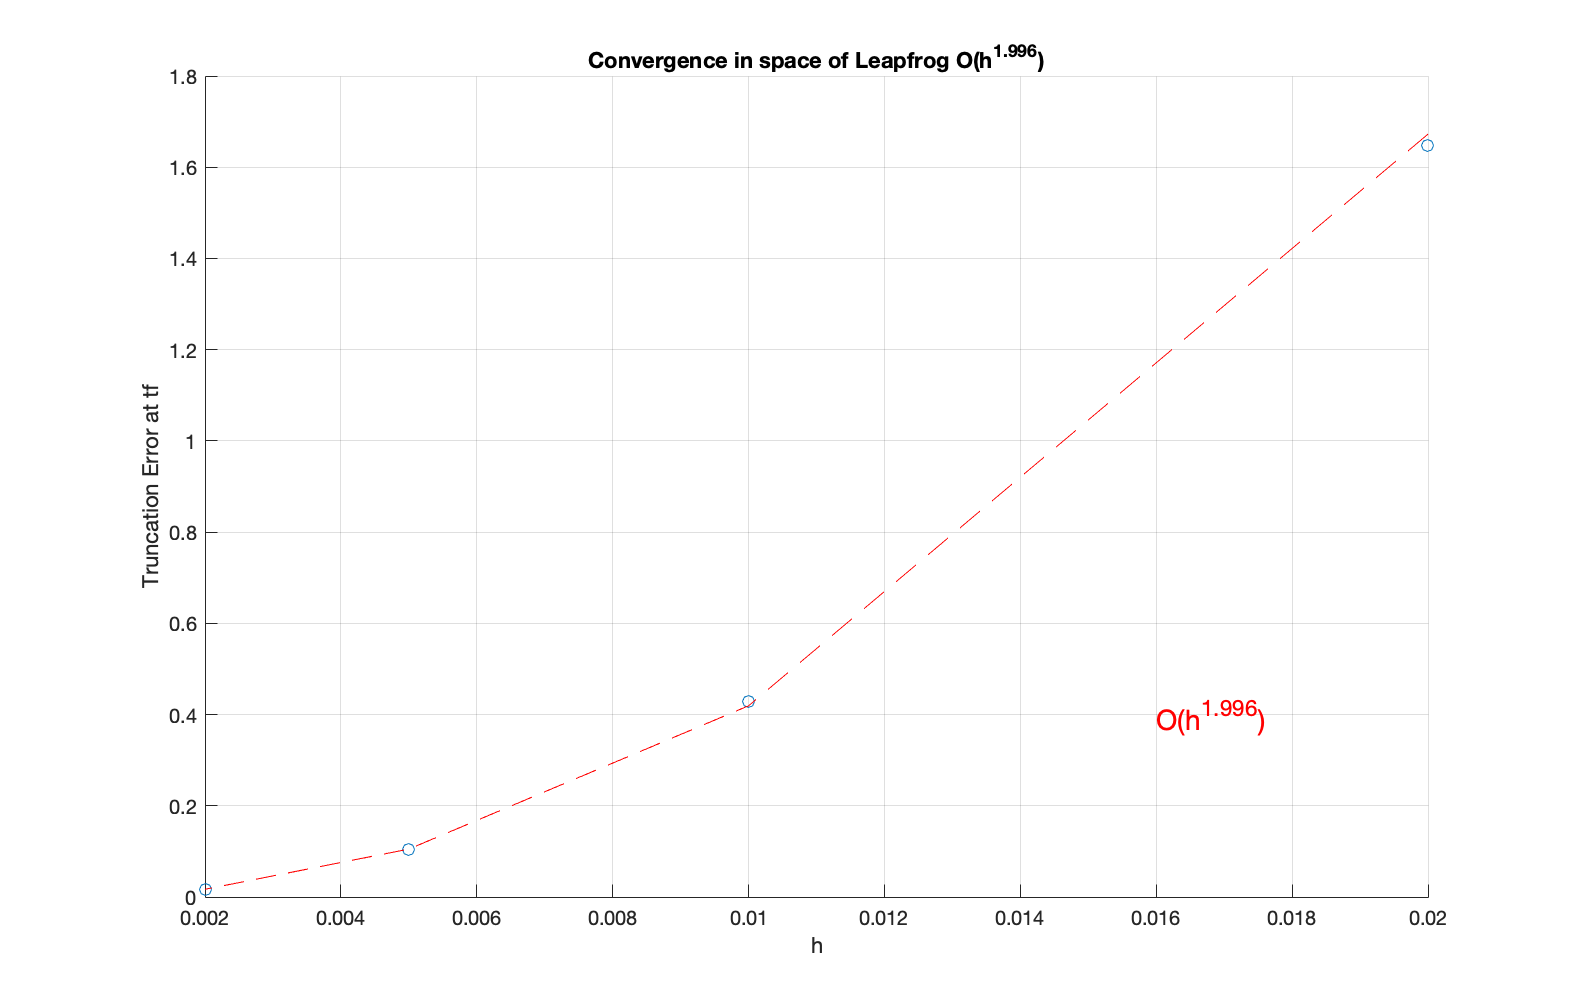
\includegraphics[width=\textwidth]{convergenceleapfrog.png}
        \end{center}
      \end{figure}


      \textbf{Code:}
      \begin{center}
        \lstinputlisting[basicstyle=\footnotesize]{gridrefinement.txt}
      \end{center}
      \vspace*{.15in}


  \end{enumerate}
  
\end{exercise}

\vspace{.15in}

\begin{exercise}{Problem P38} Consider the nonlinear Poisson equation in 2D, 
  \begin{equation*}
    u_{xx} + u_{yy} + \gamma u^3 = g(x, y)
  \end{equation*}
  on the unit square $(x, y) \in [0, 1] \times [0, 1]$, subject to zero Dirichlet boundary conditions. 

  \begin{enumerate}
    \item[\textbf{(a)}] We can manufacture a solution because we are free to choose the right-hand side $g(x, y)$. Let us define, $$u(x, y) = \sin(\pi x)\sin(2 \pi y).$$ This is a smooth function which satisfies the boundary conditions. Compute $g(x, y)$ so that $u$ is an exact solution of the differential equation. Note that the $g(x, y)$ formula will depend on $\gamma$. 
    \solution First we take the second partial derivatives of $u(x, y)$ to get $u_{xx}$ and $u_{yy}$.
    Note that $$u_{xx} = -\pi ^2\sin \left(\pi x\right)\sin \left(2\pi y\right),$$ $$u_{yy} = -4\pi ^2\sin \left(\pi x\right)\sin \left(2\pi y\right)$$
    Then by substitution we get our desired function $g(x, y)$, 
    \begin{align*}
      g(x, y) &= (-\pi^2 - 4\pi^2 + \gamma u^2)u\\
       &= (- 5\pi^2 + \gamma u^2)u
      \end{align*}
    \vspace*{.15in}

    \item[\textbf{(b)}] based on the Matlab program heat2d.m for example, write a numerical solver for the the previous problem. Use this approach:
    \begin{enumerate}
      \item Use centered differences with spacing $h_x = h_y = 1/(m+1).$
      \item Approximate the PDE by a nonlinear system, $$F(U) = 0$$ Here $U \in \RR^N$ denotes the solution of the algebraic equations, $N = m^2$, and the function $F(V)$ is the residual for a current estimate $V$.
      \item Solve the algebraic equations by Newton's method. Use $U^{[0]} = 0$ as the initial iterate. 
      \item Stop the Newton iteration when the residual norm $$|F(U^{[k]})|$$ is reduced by $10^{-9}$ of the initial residual norm. 
      \item Observe that when you set $\gamma = 0$ your code should solve the linear Poisson problem $u_{xx} + u_{yy} = g(x, y)$, by doing one Newton step. 
    \end{enumerate}
    \solution Modifying the heat2d.m code slightly we can apply the zero Dirichlet boundary conditions, and apply centered differences in both dimension. Then we need to modify the linear solve step, to do Newton's method to solve $F(U) = 0$. Writing out $F(U)$ we get the following where $A$ is the block tridiagonal matrix from discretizing in two dimensions, 
    \begin{equation*}
      F(U)= -g(x, y) + \gamma U^3 +AU
    \end{equation*}
    Since we will be performing Newton's method on this system we'll need to compute the Jacobian. Since $-g(x, y)$ is not a function of $U$, it goes away when we differentiate so we get the following,
    \begin{equation*}
      J = I3\gamma(U)^2 + A.
    \end{equation*}
    I know I can implement this very easily, by just adding a Newton method loop in the heat2d.m code in place of the linear solve. 














  \end{enumerate}
  
\end{exercise}




\end{document}











 




